%----------
%   IMPORTANTE
%----------

% Esta plantilla está basada en las recomendaciones de la guía "Trabajo fin de Grado: Escribir el TFG", que encontrarás en http://uc3m.libguides.com/TFG/escribir
% contiene recomendaciones de la Biblioteca basadas principalmente en estilos APA e IEEE, pero debes seguir siempre las orientaciones de tu Tutor de TFG y la normativa de TFG para tu titulación.



% ESTA PLANTILLA ESTÁ BASADA EN EL ESTILO IEEE


%----------
%	CONFIGURACIÓN DEL DOCUMENTO
%----------

\documentclass[12pt]{report} % fuente a 12pt

% MÁRGENES: 2,5 cm sup. e inf.; 3 cm izdo. y dcho.
\usepackage[
a4paper,
vmargin=2.5cm,
hmargin=3cm
]{geometry}

% INTERLINEADO: Estrecho (6 ptos./interlineado 1,15) o Moderado (6 ptos./interlineado 1,5)
\renewcommand{\baselinestretch}{1.15}
\parskip=6pt

% DEFINICIÓN DE COLORES para portada y listados de código
\usepackage[table]{xcolor}
\definecolor{azulUC3M}{RGB}{0,0,102}
\definecolor{gray97}{gray}{.97}
\definecolor{gray75}{gray}{.75}
\definecolor{gray45}{gray}{.45}

% Soporte para GENERAR PDF/A --es importante de cara a su inclusión en e-Archivo porque es el formato óptimo de preservación y a la generación de metadatos, tal y como se describe en http://uc3m.libguides.com/ld.php?content_id=31389625. 

% En la plantilla incluimos el archivo OUTPUT.XMPDATA. Puedes descargar este archivo e incluir los metadatos que se incorporarán al archivo PDF cuando compiles el archivo memoria.tex. Después vuelve a subirlo a tu proyecto. 
\usepackage[a-1b]{pdfx}

% ENLACES
\usepackage{hyperref}
\hypersetup{colorlinks=true,
	linkcolor=black, % enlaces a partes del documento (p.e. índice) en color negro
	urlcolor=blue} % enlaces a recursos fuera del documento en azul

% EXPRESIONES MATEMÁTICAS
\usepackage{amsmath,amssymb,amsfonts,amsthm}

% Codificación caracteres
\usepackage{txfonts} 
\usepackage[T1]{fontenc}
\usepackage[utf8]{inputenc}

% Definición idioma español
\usepackage[spanish, es-tabla]{babel} 
\usepackage[babel, spanish=spanish]{csquotes}
\AtBeginEnvironment{quote}{\small}

% diseño de PIE DE PÁGINA
\usepackage{fancyhdr}
\pagestyle{fancy}
\fancyhf{}
\renewcommand{\headrulewidth}{0pt}
\rfoot{\thepage}
\fancypagestyle{plain}{\pagestyle{fancy}}

% DISEÑO DE LOS TÍTULOS de las partes del trabajo (capítulos y epígrafes o subcapítulos)
\usepackage{titlesec}
\usepackage{titletoc}
\titleformat{\chapter}[block]
{\large\bfseries\filcenter}
{\thechapter.}
{5pt}
{\MakeUppercase}
{}
\titlespacing{\chapter}{0pt}{0pt}{*3}
\titlecontents{chapter}
[0pt]                                               
{}
{\contentsmargin{0pt}\thecontentslabel.\enspace\uppercase}
{\contentsmargin{0pt}\uppercase}                        
{\titlerule*[.7pc]{.}\contentspage}                 

\titleformat{\section}
{\bfseries}
{\thesection.}
{5pt}
{}
\titlecontents{section}
[5pt]                                               
{}
{\contentsmargin{0pt}\thecontentslabel.\enspace}
{\contentsmargin{0pt}}
{\titlerule*[.7pc]{.}\contentspage}

\titleformat{\subsection}
{\normalsize\bfseries}
{\thesubsection.}
{5pt}
{}
\titlecontents{subsection}
[10pt]                                               
{}
{\contentsmargin{0pt}                          
	\thecontentslabel.\enspace}
{\contentsmargin{0pt}}                        
{\titlerule*[.7pc]{.}\contentspage}  


% DISEÑO DE TABLAS
\usepackage{multirow} % permite combinar celdas 
\usepackage{caption} % para personalizar el título de tablas y figuras
\usepackage{floatrow} % utilizamos este paquete y sus macros \ttabbox y \ffigbox para alinear los nombres de tablas y figuras de acuerdo con el estilo definido.
\usepackage{array} % con este paquete podemos definir en la siguiente línea un nuevo tipo de columna para tablas: ancho personalizado y contenido centrado
\newcolumntype{P}[1]{>{\centering\arraybackslash}p{#1}}
\DeclareCaptionFormat{upper}{#1#2\uppercase{#3}\par}

% Diseño de tabla para ingeniería
\captionsetup*[table]{
	format=upper,
	name=TABLA,
	justification=centering,
	labelsep=period,
	width=.75\linewidth,
	labelfont=small,
	font=small
}

% DISEÑO DE FIGURAS. 
\usepackage{graphicx}
\graphicspath{{images/}} % ruta a la carpeta de imágenes

% Diseño de figuras para ingeniería
\captionsetup[figure]{
	format=hang,
	name=Fig.,
	singlelinecheck=off,
	labelsep=period,
	labelfont=small,
	font=small		
}

% NOTAS A PIE DE PÁGINA
\usepackage{chngcntr} % para numeración continua de las notas al pie
\counterwithout{footnote}{chapter}

% LISTADOS DE CÓDIGO
% soporte y estilo para listados de código. Más información en https://es.wikibooks.org/wiki/Manual_de_LaTeX/Listados_de_código/Listados_con_listings
\usepackage{listings}

% definimos un estilo de listings
\lstdefinestyle{estilo}{ frame=Ltb,
	framerule=0pt,
	aboveskip=0.5cm,
	framextopmargin=3pt,
	framexbottommargin=3pt,
	framexleftmargin=0.4cm,
	framesep=0pt,
	rulesep=.4pt,
	backgroundcolor=\color{gray97},
	rulesepcolor=\color{black},
	%
	basicstyle=\ttfamily\footnotesize,
	keywordstyle=\bfseries,
	stringstyle=\ttfamily,
	showstringspaces = false,
	commentstyle=\color{gray45},     
	%
	numbers=left,
	numbersep=15pt,
	numberstyle=\tiny,
	numberfirstline = false,
	breaklines=true,
	xleftmargin=\parindent
}

\captionsetup*[lstlisting]{font=small, labelsep=period}
% fijamos el estilo a utilizar 
\lstset{style=estilo}
\renewcommand{\lstlistingname}{\uppercase{Código}}


%BIBLIOGRAFÍA 

% CONFIGURACIÓN PARA LA BIBLIOGRAFÍA IEEE
\usepackage[backend=biber, style=ieee, isbn=false,sortcites, maxbibnames=6, minbibnames=1]{biblatex} % Configuración para el estilo de citas de IEEE, recomendado para el área de ingeniería. "maxbibnames" indica que a partir de 6 autores trunque la lista en el primero (minbibnames) y añada "et al." tal y como se utiliza en el estilo IEEE.

% Añadimos las siguientes indicaciones para mejorar la adaptación del estilos en español
\DefineBibliographyStrings{spanish}{%
	andothers = {et\addabbrvspace al\adddot}
}
\DefineBibliographyStrings{spanish}{
	url = {\adddot\space[En línea]\adddot\space Disponible en:}
}
\DefineBibliographyStrings{spanish}{
	urlseen = {Acceso:}
}
\DefineBibliographyStrings{spanish}{
	pages = {pp\adddot},
	page = {p.\adddot}
}

\addbibresource{referencias.bib} % llama al archivo referencias.bib en el que deberá estar la bibliografía utilizada


%-------------
%	DOCUMENTO
%-------------

\begin{document}
\pagenumbering{roman} % Se utilizan cifras romanas en la numeración de las páginas previas al cuerpo del trabajo
	
%----------
%	PORTADA
%----------	
\begin{titlepage}
	\begin{sffamily}
	\color{azulUC3M}
	\begin{center}
		\begin{figure}[H] %incluimos el logotipo de la Universidad
			\makebox[\textwidth][c]{
\includegraphics[width=16cm]{logo_UC3M.png}}
		\end{figure}
		\vspace{2.5cm}
		\begin{Large}
			Grado Universitario en Ingeniería Informática\\			
			 2020-2021\\ %Indica el curso académico
			\vspace{2cm}		
			\textsl{Trabajo Fin de Grado}
			\bigskip
			
		\end{Large}
		 	{\Huge ``Reconocimiento de Emociones en los Acompañantes de un Vehículo''}\\
		 	\vspace*{0.5cm}
	 		\rule{10.5cm}{0.1mm}\\
			\vspace*{0.9cm}
			{\LARGE Binxian Huang}\\ 
			\vspace*{1cm}
		\begin{Large}
			Tutor/es\\
			Jose Antonio Iglesias Martínez\\
			Leganés, Junio 2024\\
		\end{Large}
	\end{center}
	\vfill
	\color{black}
	% SI NUESTRO TRABAJO SE VA A PUBLICAR CON UNA LICENCIA CREATIVE COMMONS, INCLUIR ESTAS LÍNEAS. ES LA OPCIÓN RECOMENDADA.
	
\includegraphics[width=4.2cm]{creativecommons.png}\\ %incluimos el logotipo de Creative Commons
	Esta obra se encuentra sujeta a la licencia Creative Commons \textbf{Reconocimiento - No Comercial - Sin Obra Derivada}
	\end{sffamily}
\end{titlepage}

\newpage %página en blanco o de cortesía
\thispagestyle{empty}
\mbox{}

%----------
%	RESUMEN Y PALABRAS CLAVE
%----------	
\renewcommand\abstractname{\large\bfseries\filcenter\uppercase{Resumen}}
\begin{abstract}
\thispagestyle{plain}
\setcounter{page}{3}
	
	% ESCRIBIR EL RESUMEN AQUÍ
	
	\textbf{Palabras clave:}
	% Escribir las palabras clave aquí
	
	\vfill
\end{abstract}
	\newpage % página en blanco o de cortesía
	\thispagestyle{empty}
	\mbox{}


%----------
%	DEDICATORIA
%----------	
\chapter*{Dedicatoria} % \chapter* evita que aparezca en el índice

\setcounter{page}{5}
	
	% ESCRIBIR LA DEDICATORIA AQUÍ	
		
	\vfill
	
	\newpage % página en blanco o de cortesía
	\thispagestyle{empty}
	\mbox{}
	

%----------
%	ÍNDICES
%----------	

%--
% Índice general
%-
\tableofcontents
\thispagestyle{fancy}

\newpage % página en blanco o de cortesía
\thispagestyle{empty}
\mbox{}

%--
% Índice de figuras. Si no se incluyen, comenta las líneas siguientes
%-
\listoffigures
\thispagestyle{fancy}

\newpage % página en blanco o de cortesía
\thispagestyle{empty}
\mbox{}

%--
% Índice de tablas. Si no se incluyen, comenta las líneas siguientes
%-
\listoftables
\thispagestyle{fancy}

\newpage % página en blanco o de cortesía
\thispagestyle{empty}
\mbox{}


%----------
%	MEMORIA
%----------	
\clearpage
\pagenumbering{arabic} % numeración con números arábigos para el resto de la memoria.	



	% COMENZAR A ESCRIBIR la MEMORIA
	
	% IMPORTANTE: en LaTeX hay una serie de caracteres especiales, que son: # $ % & \ ^ _ { } ~. Si aparecen en el texto, tendrás un error al compilar. La mayoría se pueden escapar escribiendo \ delante. Para \ utiliza \textbackslash ; para ^ \textasciitilde y para ~ \textasciicircum.

    % COMO incluir una FIGURA siguiendo las recomendaciones de la Guía: Alineación del título: izquierda, en la parte inferior de la figura; fuente a 10pt (el resto de la memoria está a 12); Numeración de la figura: se identificarán con números arábigos consecutivos tras la palabra Tabla. Si se sigue un esquema numérico de capítulos, el número de la tabla debe identificar con su primer dígito al capítulo, seguido por un punto y el número consecutivo que corresponda (Tabla 1.1, etc.); Propiedad intelectual: Se debe indicar la fuente de origen de la información en la parte inferior de la figura, a continuación del título.
    
    % EJEMPLO DE INCLUSIÓN de una figura:
    % \begin{figure}[H]
    % 	\ffigbox[\FBwidth] {
    % 	\caption[Nombre que aparecerá en el índice]{Nombre que aparecerá debajo de la figura}
    % 	}
    % 	{\includegraphics[scale=0.6]{archivo de la imagen; deberá estar en la carpeta de imágenes}}
    % \end{figure}
    
    % COMO incluir una TABLA siguiendo las recomendaciones de la Guía: Alineación del título: Centrado en la parte superior de de la tabla, en la parte superior de la tabla; fuente a 10pt (el resto de la memoria está a 12) y en mayúsculas; Numeración: se identificarán con números arábigos consecutivos tras la palabra Tabla. Si se sigue un esquema numérico de capítulos, el número de la tabla debe identificar con su primer dígito al capítulo, seguido por un punto y el número consecutivo que corresponda (Tabla 1.1, etc.); Propiedad intelectual: Se debe indicar la fuente de origen de la información en la parte inferior de la tabla.
    
    % EJEMPLO DE INCLUSIÓN de una tabla:
% \begin{table}[H]
% 	\ttabbox[\FBwidth]
% 	{\caption{Lorem ipsum}}
% 	{\begin{tabular}{|c|P{1.5cm}|c|P{1.5cm}|P{2cm}|c|P{1.5cm}|P{2cm}|}
% 		\hline
% 		\multicolumn{2}{|c|}{\textbf{I}} & \multicolumn{2}{c|}{\textbf{II}} & \multicolumn{3}{c|}{\textbf{III}} & \textbf{IV} \\
% 		\hline
% 		x & y & x & y & x & y & x & y \\
% 		\hline
% 		10.0 & 8.04 & 10.0 & 9.14 & 10.0 & 7.46 & 8.0 & 6.58 \\
% 		\hline
% 		8.0 & 6.95 & 8.0 & 8.14 & 8.0 & 6.77 & 8.0 & 5.76 \\
% 		\hline
% 		13.0 & 7.58 & 13.0 & 8.74 & 13.0 & 12.74 & 8.0 & 7.71 \\
% 		\hline
% 		9.0 & 8.81 & 9.0 & 8.77 & 9.0 & 7.11 & 8.0 & 8.84 \\
% 		\hline
% 		11.0 & 8.33 & 11.0 & 9.26 & 11.0 & 7.81 & 8.0 & 8.47 \\
% 		\hline
% 		14.0 & 9.96 & 14.0 & 8.10 & 14.0 & 8.84 & 8.0 & 7.04 \\
% 		\hline
% 		6.0 & 7.24 & 6.0 & 6.13 & 6.0 & 6.08 & 8.0 & 5.25 \\
% 		\hline
% 		4.0 & 4.26 & 4.0 & 3.10 & 4.0 & 5.39 & 19.0 & 12.50 \\
% 		\hline
% 		12.0 & 10.84 & 12.0 & 9.13 & 12.0 & 8.15 & 8.0 & 5.56 \\
% 		\hline
% 		7.0 & 4.82 & 7.0 & 7.26 & 7.0 & 6.42 & 8.0 & 7.91 \\
% 		\hline
% 		5.0 & 5.68 & 5.0 & 4.74 & 5.0 & 5.73 & 8.0 & 6.89 \\
% 		\hline
% 		\multicolumn{5}{l}{Fuente: BOE}
% 	\end{tabular}}
% \end{table}



\chapter{Introducción}

\section{Motivación}

Actualmente, siendo una era de grandes avances tecnológicos, la industria automotriz destaca como un faro de innovación, particularmente en el desarrollo de sistemas inteligentes diseñados para mejorar la seguridad y personalizar la experiencia del conductor. La integración de la Inteligencia Artificial (IA) en los sistemas de los vehículos representan un cambio transformador, pasando de los vehículos tradicionales a los “vehículos inteligentes” o smart vehicles. Estos vehículos no son meros medios de transporte, sino que son plataformas sofisticadas que se adaptan de forma dinámica a las necesidades y estados emocionales de los pasajeros. 

Las tecnologías en los vehículos actuales en gran medida no tienen en cuenta el contexto emocional de los pasajeros, dependen de una entrada en concreto como comandos táctiles o vocales. La implementación de sistemas capaces de percibir y reaccionar a los estados emocionales de los pasajeros podría ser un gran avance para el sector del diseño de software centrado en el usuario.

Este proyecto se centra en aprovechar el gran avance de la IA para desarrollar un modelo capaz de reconocer y analizar emociones faciales de los pasajeros en tiempo real, y aplicarlo en un sistema afectando a la forma en la que los vehículos interactúan con los ocupantes, ajustando configuraciones internas como la música, la iluminación y la temperatura, para mejorar el confort y la seguridad. Esto serviría mejorar la experiencia del usuario, además de que podría ser útil en los “Sistemas Avanzados de Ayuda a la Conducción” o Advanced Driver-Assistance System (ADAS), ya que ayudaría al conductor a librarse se realizar por sí mismo dichas acciones y no distraerse de la conducción, además que el modelo realizado también podría ser utilizado en los sistemas. 

\section{Objetivos}

El objetivo principal de este proyecto es desarrollar un modelo de reconocimiento de emociones faciales, que pueda ser aplicado en el sistema de un vehículo para mejorar la experiencia del usuario. Para ello, se plantean los siguientes objetivos específicos:

\begin{itemize}

	\item Desarrollar un modelo capaz de identificar las expresiones faciales mediante imágenes de las caras de los pasajeros.
    \item Diseñar un sistema que permita integrar el modelo con los demás sistemas del vehículo, además de poder interactuar con los controles del vehículo como la iluminación, los sistemas de audio o el control del clima.
    \item Mejorar las medidas de seguridad en función de los resultados del modelo, como permitir al sistema ajustar la dinámica de conducción, activar protocolos de seguridad, alertar sobre posibles peligros, etc. si se detectan señales de enfado o angustia. 
    \item Análisis y estudio de viabilidad económica y técnica del sistema, verificando si la integración de esta tecnología es factible para el mercado comercial, además de un análisis de impacto y una evaluación de los usuarios en la aceptación de esta tecnología en los vehículos.

\end{itemize}

\section{Estructura de la memoria}

El documento se organiza en siete capítulos principales:

\begin{enumerate}

    \item \textbf{Introducción:} En este capítulo se describe el contexto general del proyecto, incluyendo la motivación que impulsa a su realización y los objetivos específicos que se pretende alcanzar.
    \item \textbf{Estado del Arte:} En este capítulo se presenta una breve revisión literaria de los temas relacionados al proyecto, los avances de la experiencia del usuario el sector de los automóviles, la inteligencia artificial en la industria de la automoción, los ADAS y los sistemas implementados que mejoran las experiencias de los usuarios, además de un análisis de los  distintos trabajos previos en relación al tema. 
    \item \textbf{Diseño del sistema:} En este capítulo se describe el diseño y arquitectura del sistema, los requisitos necesarios, un análisis y explicación de la fuente de datos elegida para la realización del modelo, al igual que una descripción de las metodologías y herramientas que se usarán. 
    \item \textbf{Implementación y resultados:} En este capítulo se documenta el proceso práctico de la realización del modelo así como un análisis de los resultados obtenidos.
    \item \textbf{Marco regulador:} En este capítulo se realiza una revisión de las normativas y regulaciones relevantes que afecten a este proyecto. 
    \item \textbf{Entorno socio-económico:} En este capítulo se describe en una primera sección la planificación y administración del proyecto, y en una segunda sección el posible impacto del proyecto en la sociedad y la economía.

\end{enumerate}



\chapter{Estado del arte}

\section{Experiencia del Usuario en la Industria de la Automoción}

La experiencia de usuario (UX) es un concepto fundamental en el ámbito del diseño y desarrollo de productos y servicios, y su importancia ha ido creciendo exponencialmente en los últimos años. En el contexto de la industria automotriz, la UX se refiere a la manera que interactúan los usuarios con los vehículos, las tecnologías que incorporan estos mismos, y cómo esas interacciones afectan a la satisfacción del usuario.
\cite{userExperience}

Una buena experiencia de usuario no sólo implica una simple funcionalidad, ya sea ergonomía del asiento, integración de sistemas de entretenimiento, o características que mejoran la seguridad y comodidad; también implica tener en cuenta aspectos emocionales y psicológicos que influyen en la decisión de compra y la marca, como la facilidad de uso o la intuitividad de las interfaces de usuario. 

Al crecer la expectativa de los usuarios para una experiencia mejor y personalizable, conlleva a los fabricantes a tomar importancia el diseño centrado en el usuario con la realización de investigaciones de mercado y pruebas de usuario para comprender sus necesidades y deseos, lo que es beneficioso para la innovación y competitividad del sector. 

\subsection{Panales táctiles}

La interacción con los componentes de un automóvil moderno es muy diferente en comparación con unas décadas atrás. En el pasado, los paneles de los coches solo contenían controles físicos sencillos y la interacción era mediante botones, diales y deslizadores para ajustar la radio o el aire acondicionado. Además, las radios solo funcionaban mediante dispositivos físicos como casetes o CDs. Posteriormente evolucionaron a pequeñas pantallas digitales que añadían una funcionalidad de GPS muy sencilla, hasta evolucionar a lo que hay actualmente, pantallas táctiles que sustituyen e incluyen la mayoría de las funcionalidades de los botones físicos.
\cite{touchScreen}

\begin{figure}[h]
    \centering
    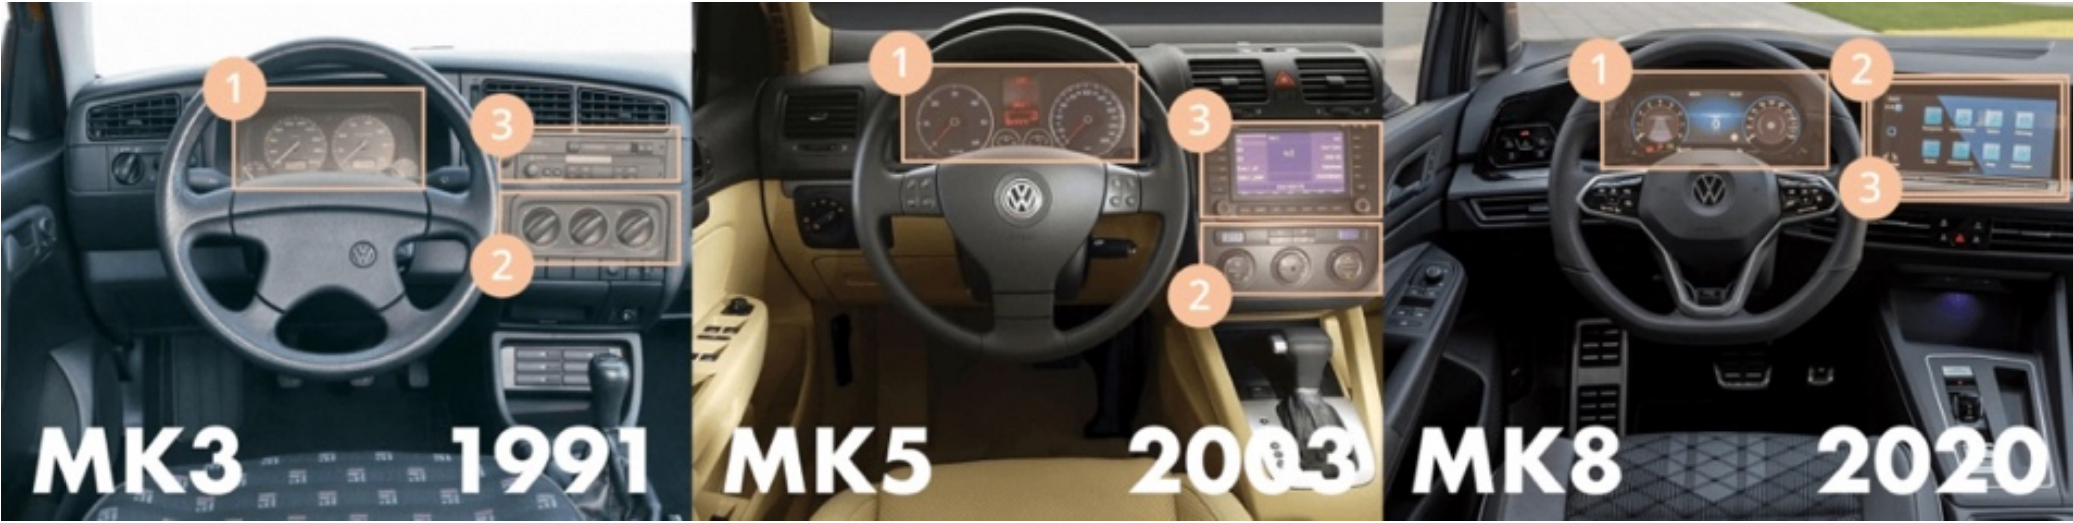
\includegraphics[width=0.9\textwidth]{evolutionTouchscreen.png}
    \caption{Evolución del panel en un Volkswagen Golf \cite{userExperience}.}
    \label{fig:imagen1}
\end{figure}

Esta adaptación es debido al ràpido avance tecnológico de los teléfonos móviles y tablets, la comodidad en la que se interactúa pulsando o deslizando sobre las pantallas de los dispositivos, es lo que ha promovido a los fabricantes de automóviles a incorporar las mismas características de las pantallas táctiles en el lugar de los controles físicos de los coches.  

\begin{figure}[h]
    \centering
    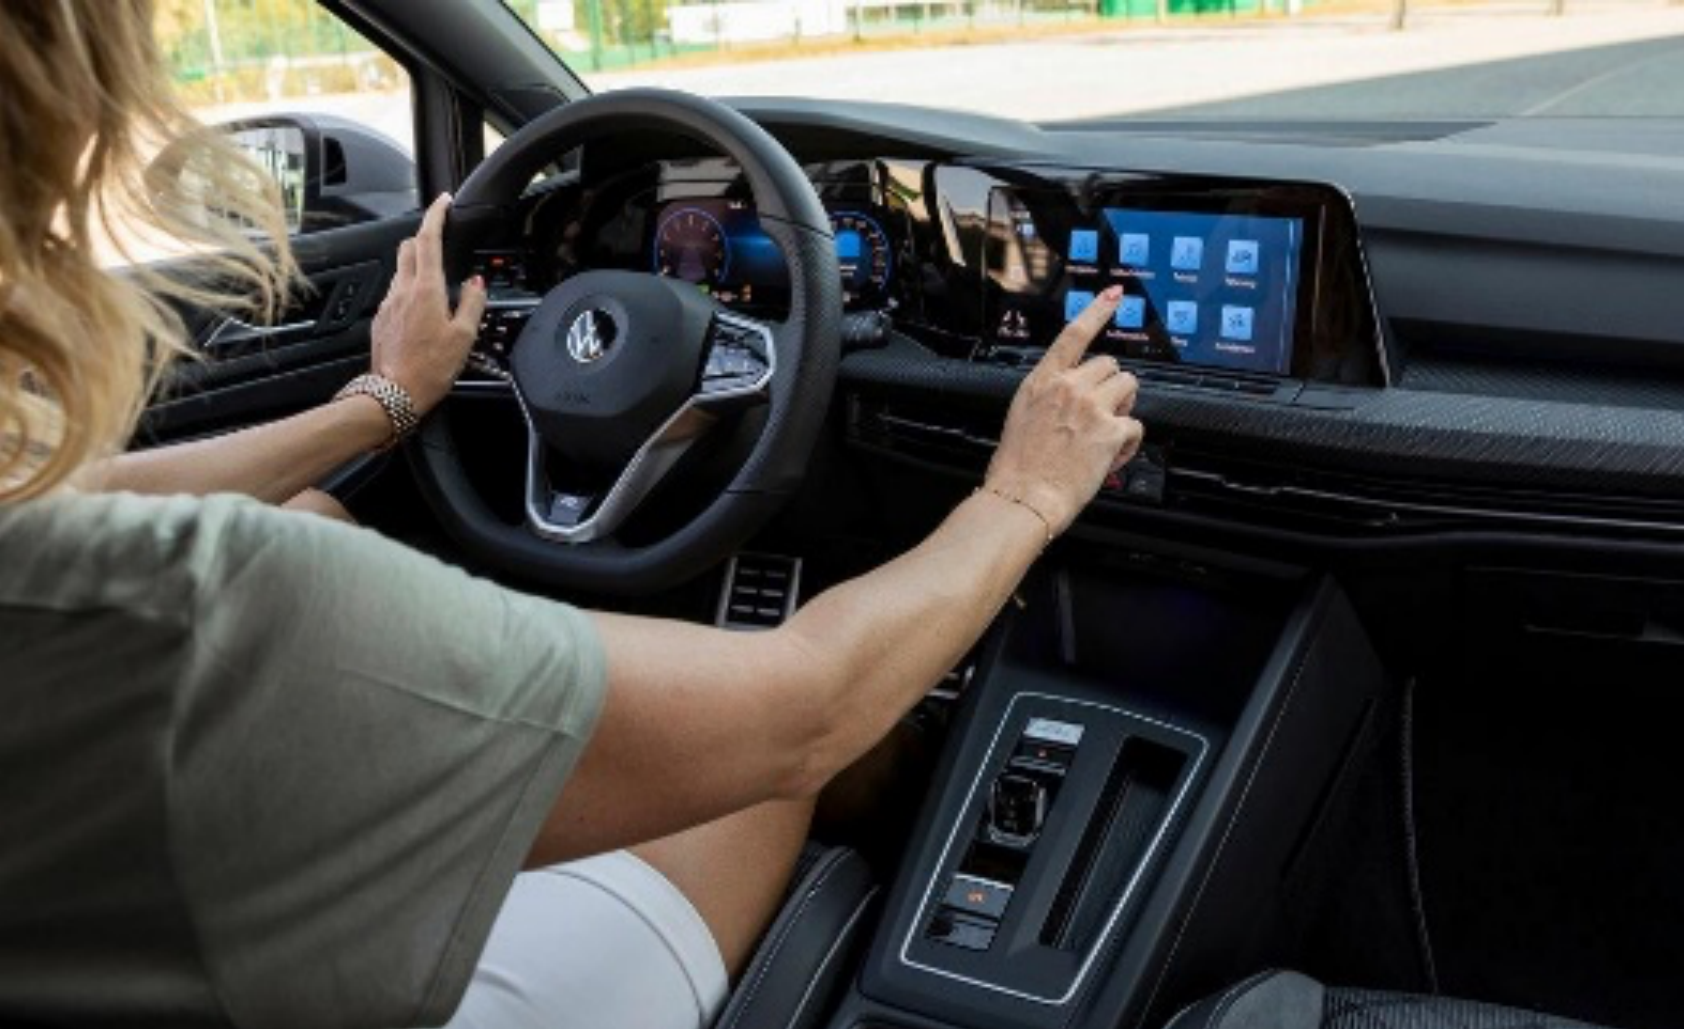
\includegraphics[width=0.9\textwidth]{usingTouchscreen.png}
    \caption{Conductor interaccionando con una pantalla táctil \cite{userExperience}.}
    \label{fig:imagen2}
\end{figure}

Las pantallas táctiles aportan bastantes beneficios, como pueden ser un diseño limpio y simplificado, siendo visualmente más atractivo al no contener tantos botones y diales, o flexibilidad y dinamicidad el la interfaz para añadir o mejorar funcionalidades.

Sin embargo, aunque permiten una interacción más sencilla y limpia, también presentan problemas de seguridad hacia el conductor. La distracción visual del conductor por la necesidad de desviar la vista de la carretera para interactuar con los paneles, lo que podría aumentar el riesgo de accidente o una falta de retroalimentación para las acciones que se realicen dificultaría al usuario manejar la pantalla sin mirar. Incluso en países como Reino Unido donde los vehículos tienen los volantes a la derecha, interaccionar con la pantalla con la mano izquierda podría ser difícil o incómodo. 

\subsection{Coches conectados}

El concepto de “coche conectado” surge de la integración de los coches en el Internet de las Cosas (IoT), al ser capaces de acceder a Internet, comunicarse con dispositivos inteligentes y recopilar datos en tiempo real. Inicialmente los automóviles contenían un número pequeño de Unidades de Control Electrónico (ECU), donde cada una era independiente de otra y realizaba una funcionalidad simple. Los coches de hoy en día pueden contener hasta 70 ECUs realizando muchas funcionalidades variadas, además de poder utilizar protocolos de comunicación que les permiten “hablar” con otros vehículos e infraestructuras, e incluso con Internet. Actualmente, incluso se ha logrado la integración de dispositivos móviles y smartphones en los paneles de los automóviles ofreciendo servicios avanzados de multimedia y entretenimiento. 
\cite{mobileIntegration}

\begin{figure}[h]
    \centering
    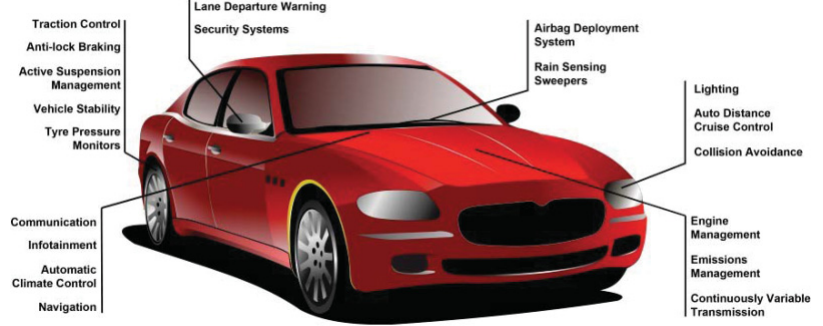
\includegraphics[width=0.9\textwidth]{ecu.png}
    \caption{Ejemplos de ECUs en un coche \cite{mobileIntegration}.}
    \label{fig:imagen3}
\end{figure}

\begin{figure}[H]
    \centering
    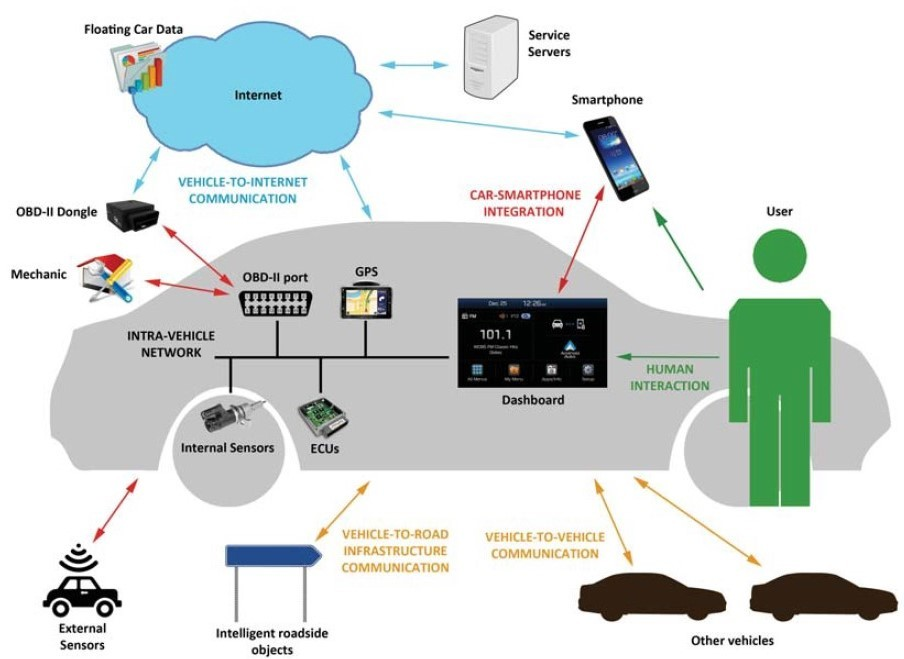
\includegraphics[width=0.9\textwidth]{connected_car_system.jpg}
	\caption{Visión general de un sistema de coche conectado \cite{mobileIntegration}.}
    \label{fig:imagen4}
\end{figure}

Al tener tantos dispositivos interconectados, las tecnologías y protocolos de comunicación en los coches conectados son fundamentales para su correcto funcionamiento, ya que permiten la interacción entre los componentes del vehículo, otros vehículos o las infraestructuras de las vías. Los diferentes tipos de comunicación que un coche conectado debe garantizar y las tecnologías disponibles para realizar dichas conexiones son las siguientes: 

\begin{itemize}

    \item \textbf{Vehicle To Sensors On Board communication (V2S) o Comunicación Intra-Vehicular:} esta comunicación se centra en la transmisión de información entre las ECUs y los sensores del vehículo, y se realiza mediante cables físicos o redes inalámbricas como Bluetooth o Ultra-Wideband. Un detalle a tener en cuenta es que aunque las redes inalámbricas ofrecen más versatilidad, presentan todavía problemas de seguridad y fiabilidad.
    \item \textbf{Vehicle To Vehicle Communication (V2V) o Comunicación Inter-Vehicular:} esta comunicación se centra en la transmisión de información entre diferentes coches sin la necesidad de un dispositivo remoto centralizado, utilizada principalmente para evitar accidentes, optimizar de rutas, compartir información multimedia y facilitar la interacción social entre conductores. Esta tecnología de comunicación enfrenta todavía desafíos ya una constante variación en la topología de la red o la presencia de obstáculos puede dificultar su gestión o interrupciones en el flujo de los datos.
    \item \textbf{Vehicle To Road Infrastructure Communication (V2R):} esta comunicación se centra en la transmisión de información entre un vehículo y una infraestructura de la vía compuesta por señales de tráfico, sensores de carretera y semáforos, y utilizada principalmente para una gestión eficiente del tráfico.
    \item \textbf{Vehicle To Internet Communication (V2I):} esta comunicación se centra en la transmisión de información entre un vehículo e Internet, utilizada principalmente para interaccionar con sus servicios y acceder a información multimedia. Se realiza mediante infraestructuras de red celular, al igual que un dispositivo móvil, utilizando una tarjeta SIM para permitir que el vehículo se conecte a una red 3G o 4G.

\end{itemize}

En cuanto a la integración de dispositivos móviles y smartphones con los coches conectados, se han desarrollado soluciones software capaces de permitir a la pantalla del coche acceder a los datos del dispositivo, e incluso permite al usuario controlar aplicaciones del dispositivo en la pantalla. Esta integración ofrece varias ventajas, como pueden ser una personalización diferente para cada usuario que depende de cada dispositivo, o además facilitar a los desarrolladores de aplicaciones crear aplicaciones sobre una plataforma genérica en vez de un modelo de pantalla específico. Las soluciones de integración más extendidas son: 

\begin{itemize}

    \item \textbf{MirrorLink:} desarrollado por el Car Connectivity Consortium (CCC), y permite la conexión mediante USB o Wi-Fi Direct. Crea directrices para la interfaz gráfica de las aplicaciones, con iconos de gran tamaño facilitando una navegación rápida y sencilla.
    \item \textbf{Applink:} desarrollada por Ford, y permite realizar distintas acciones dentro del vehículo como mostrar mensajes en la pantalla, reproducir música y ofrecer controles por voz.
    \item \textbf{Apple CarPlay:} solución desarrollada para dispositivos iPhone, extendiendo las funcionalidades del sistema estándar del vehículo, y permite controlar aplicaciones mediante la pantalla, comandos de voz con SIRI, y llamadas y mensajes con manos libres.
    \item \textbf{Android Auto:} solución desarrollada por la Open Automotive Alliance, y centrada en la conexión con dispositivos Android. Proporciona un tablero simple que permite el acceso a sistemas de navegación, como por ejemplo Google Maps, además de música, llamadas telefónicas, comandos de voz, etc.

\end{itemize}

\begin{figure}[h]
	\centering
	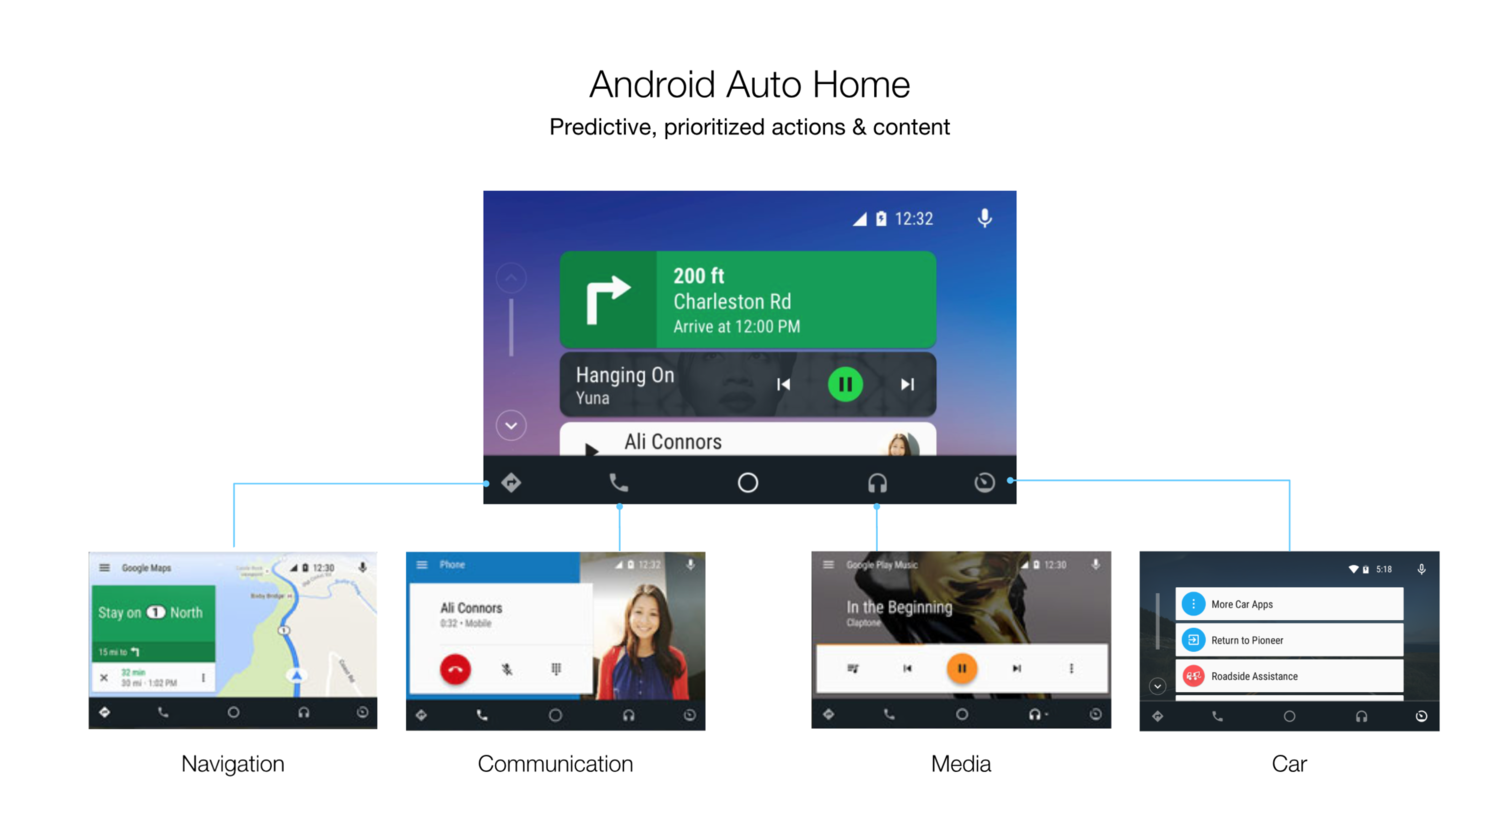
\includegraphics[width=0.9\textwidth]{androidAuto.png}
	\caption{Ejemplos de interfaces de Android Auto en la pantalla del coche.}
	\label{fig:imagen5}
\end{figure}

Actualmente, de las tecnologías anteriores las más populares y mayoritariamente implementadas  son las dos últimas,  Apple CarPlay y Android Auto, debido a que tienen un mayor número de funcionalidades y tienen un mayor número de dispositivos con dicho sistema operativo compatible.

\begin{figure}[h]
    \centering
    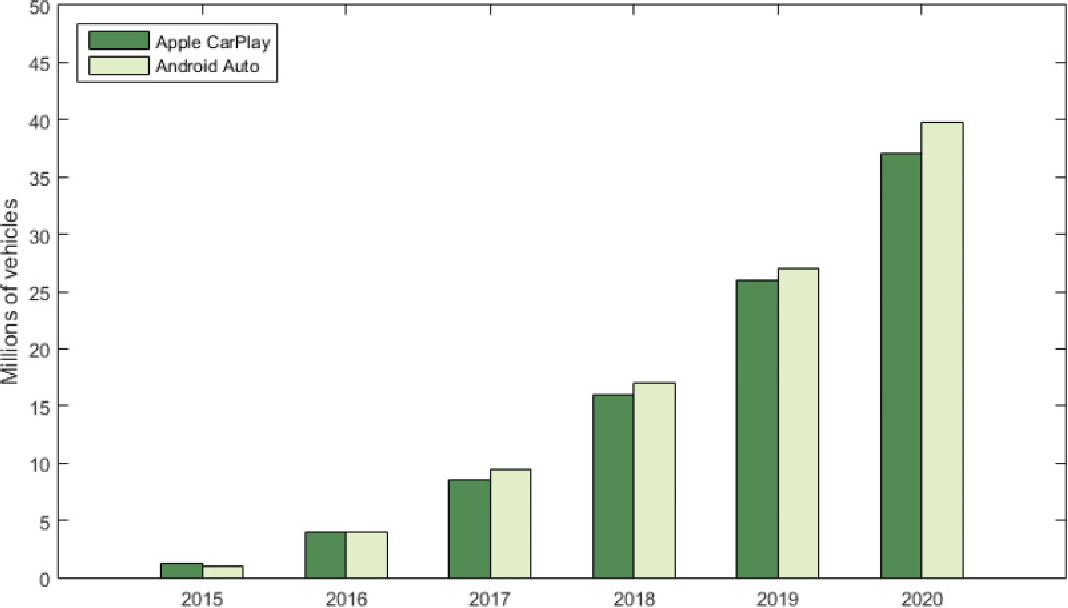
\includegraphics[width=0.9\textwidth]{integrationSolution.png}
	\caption{Ventas de coches con Apple CarPlay vs Android Auto \cite{mobileIntegration}.}
	\label{fig:imagen6}
\end{figure}

\subsection{Heads Up Display (HUD)}



\section{Sistemas Avanzados de Ayuda a la Conducción (ADAS)}



\section{Vehículos Autónomos}



\section{Inteligencia Artificial y Aprendizaje Automático}



\section{Trabajos Relacionados}



\chapter{Diseño del sistema}



\chapter{Implementación y resultados}



\chapter{Marco regulador}



\chapter{Entorno socio-económico}

\section{Gestión del proyecto}



\section{Impacto socio-económico}



\chapter{Conclusiones y trabajos futuros}


%----------
%	BIBLIOGRAFÍA
%----------	

%\nocite{*} % Si quieres que aparezcan en la bibliografía todos los documentos que la componen (también los que no estén citados en el texto) descomenta está línea

\clearpage
\addcontentsline{toc}{chapter}{Bibliografía}
\setquotestyle[english]{british} % Cambiamos el tipo de cita porque en el estilo IEEE se usan las comillas inglesas.
\printbibliography



%----------
%	ANEXOS
%----------	

% Si tu trabajo incluye anexos, puedes descomentar las siguientes líneas
%\chapter* {Anexo x}
%\pagenumbering{gobble} % Las páginas de los anexos no se numeran



\end{document}